%\documentclass[a4paper,12pt]{report}
\documentclass[a4paper,12pt]{article}
%\documentclass[a4paper,12pt]{book}
\usepackage{polski}
\usepackage[polish]{babel}
\usepackage[utf8]{inputenc}
\usepackage[top=2.5cm, bottom=2.5cm, left=3cm, right=2.5cm]{geometry}
\usepackage[justification=centering]{caption}
\usepackage{graphicx}
\usepackage{setspace}
\usepackage{ifthen}
\usepackage{a4wide}
\usepackage{fullpage}
\usepackage{verbatim}
\usepackage[usenames,dvipsnames]{color}
\usepackage{hyperref}
\usepackage{subfig}
\usepackage{listings}
\usepackage{mdwlist}
\usepackage{titlesec}
\usepackage{lipsum}
\usepackage{multirow}
\usepackage{enumitem}
\usepackage[clock]{ifsym}
\usepackage{clock}
\usepackage{amsmath}
\usepackage{cite}

\usepackage{pgfplots}
\usepackage{tikz}
\usetikzlibrary{automata,positioning,shapes,shadows,arrows,backgrounds,trees,fit,calc,decorations.pathreplacing,decorations.markings}

\hypersetup{
%	bookmarks=true,
	pdftitle={ELAN},
	pdfauthor={Damian Karbowiak, Grzegorz Powała},
	pdfsubject={ELAN},
	pdfkeywords={Politechnika Śląska ELAN},
	colorlinks=true,
	linkcolor=black,
	citecolor=black,
	urlcolor=black
	}
	
\let\subsubsubsection\paragraph
%\setcounter{secnumdepth}{6} % subsubparagraph ???
% that is, subsubsubsubsubsection :-)
\setcounter{secnumdepth}{4}

\newcommand{\tytul}{Projekt i realizacja stanowiska laboratoryjnego do badania zależności czasowych w sieci EtherCAT}
\newcommand{\data}{\today}
\newcommand{\promotor}{dr~inż. Jacek Stój}
\newcommand{\autor}{inż. Damian Karbowiak}
\newcommand{\konsultant}{}

\titlespacing{\section}{1cm}{*4}{*1.5}
\titlespacing{\subsection}{1cm}{*4}{*1.5}
\titlespacing{\subsubsection}{1cm}{*4}{*1.5}

\setitemize{itemsep=0pt, topsep=2pt}
\setenumerate{itemsep=0pt, topsep=2pt}

\linespread{1.3}

\begin{document}

\lstset{backgroundcolor=\color{white}, boxpos=c, captionpos=b}
\lstset{numbers=left, stepnumber=1, numbersep=10pt, frame=single}
\lstset{frameround=tttt}
\renewcommand{\lstlistlistingname}{\vspace*{-13mm}}
\renewcommand{\listfigurename}{\vspace*{-13mm}}
%\renewcommand*\l@figure[2]{\indent}
\renewcommand{\listtablename}{\vspace*{-13mm}}
\renewcommand*{\refname}{\vspace*{-13mm}}
\renewcommand{\lstlistingname}{Kod źródłowy} 

\newcommand{\rowstyle}[1]{\gdef\currentrowstyle{#1}%
#1\ignorespaces
}

%\begin{abstract}
\thispagestyle{plain}
\pagenumbering{Roman}
\noindent Damian KARBOWIAK, Grzegorz POWAŁA \\
Opiekun naukowy: dr inż Jacek STÓJ
\begin{center}
\textbf{Zastosowanie protokołu ELAN w sieci pomiarowej}
\end{center}
\textbf{Streszczenie: }
Niniejszy artykuł opisuje wynik realizacji aplikacji do gromadzenia danych z analizatorów składu gazu firmy SIEMENS.
W artykule przedstawione zostało rozwiązanie zaproponowane i zaimplementowane przez autorów niniejszej publikacji. \\
\textbf{Słowa kluczowe: } ELAN, Siemens, pomiary, analizator gazów
\begin{center}
\textbf{Application of ELAN protocol in measurement network}
\end{center}
\textbf{Summary: }
This article describe result of realisation application to collect data from gas analyzers by SIEMENS company.\\
\textbf{Keywords: } ELAN, Siemens, measurement, gas analyzer
\clearpage
%\end{abstract}

\pagenumbering{arabic}
\tableofcontents
\addtocontents{toc}{\protect\vspace*{.05\baselineskip}}
\clearpage

\section{Opis protokołu ELAN}

ELAN (ang. Economical Local Area Network), czyli ekonomiczna sieć lokalna został wprowadzony przez firmę SIEMENS w swoich analizatorach składu gazu. Protokół ten według twórców został wprowadzony jako ekonomiczny interfejs szeregowy do transmisji wartości mierzonych pomiędzy analizatorami oraz prostej komunikacji z komputerami PC dla celów testowych i serwisowych. Najważniejsze parametry zebrano w Tablicy~\ref{tab:parametry}.
Zostało wprowadzone ograniczenie maksymalnej liczby urządzeń pracujących w sieci do 14 (2 urządzenia kontrolne/komputery oraz do 12 analizatorów). Obsługiwane analizatory firmy SIEMENS:
\begin{itemize}
\item ULTRAMAT 6
\item OXYMAT 6 / OXYMAT 61
\item CALOMAT 6
\item ULTRAMAT 23
\end{itemize}
Komunikacja została oparta na następujących założeniach:
\begin{itemize}
\item Wszystkie podpięte analizatory mają te same prawa
\item Aby uniknąć konfliktów, każdy analizator musi sprawdzić stan magistrali i zatrzymać transmisję natychmiast w razie potrzeby (mechanizm CSMA / CD)
\item Nowa komenda może zostać wysłana dopiero gdy poprzednia komenda zostanie potwierdzona (z wyjątkiem trybu rozgłoszeniowego)
\end{itemize}

\begin{table}[h]
\centering
\begin{tabular}{|l|l|}
\hline Poziom & RS485 \\ 
\hline Szybkość transmisji & 9600 \\ 
\hline Bity danych & 8 \\ 
\hline Bit startu & 1 \\ 
\hline Bit stopu & 1 \\ 
\hline Kontrola parzystości & nie \\ 
\hline no ECHO &  \\ 
\hline 
\end{tabular} 
\caption{Parametry interfejsu}
\label{tab:parametry}
\end{table}

%\subsection{Analiza statystyczna protokołu}
%TCS -- Rozmiar transmitowanego znaku (ang. transmitted char size)\\
%CS -- rozmiar znaku (ang. char size)\\
%SpB -- bit stopu (ang. Stop bit) \\
%StB -- bit startu (ang. Start bit)
%$$TCS = CS + StB + SpB= 8+1+1=10 [b]$$
%CPS -- liczba znaków na sekundę (ang. chars per second) \\
%CBR -- znakowa szybkość transmisji (ang. char baud rate) \\
%BR -- szybkość transmisji (ang. baud rate) \\
%Szybkość transmisji wg dokumentacji: 9600 bps (bitów na sekundę)
%$$CBR=BR/TCS=9600/10=960 [cps]$$

\subsection{Ramka}
Każda ramka w sieci wygląda ogólnie jak na Rysunku~\ref{elan:ramka}. W pierwszej wersji, aktualnie zrealizowanej przez autorów obsługiwane są jedynie ramki rozgłoszeniowe, wykorzystujące komendę 'k', 2.
\begin{figure}[htbp]
 \centering
        \tikzstyle{background grid}=[draw, black!50,step=.25cm]
	\begin{tikzpicture}[node distance=1.5mm, auto]%, show background grid]
	\tikzset{
    	mynode/.style={rectangle,rounded corners,draw=black, top color=white, very thick, inner sep=4mm, 		text centered,font=\footnotesize},
    	mynodemini/.style={rectangle,rounded corners,draw=black, top color=white, thick, inner sep=2mm, text centered,font=\scriptsize},    	
	    myarrow/.style={->, >=latex', shorten >=1pt, ultra thick},
	    myline/.style={-, =latex', shorten >=1pt, rounded corners, ultra thick},
	    mylabel/.style={text centered, font=\scriptsize\bfseries} 
	} 
	\node[bottom color=gray!50, mynode, text width=2.3cm] (start) {Start};  
	\node[bottom color=gray!50, mynodemini, below=of start.213, text width=1cm] (dle) {DLE (10H)};	
	\node[bottom color=gray!50, mynodemini, right=of dle, text width=1cm] (soh) {SOH (01H)};  
	
	\node[bottom color=yellow!50, mynode, right=of start, text width=6.3cm] (used_data) {USED DATA};
	\node[bottom color=yellow!50, mynodemini, below=of used_data.190] (ud1) {TA};  	 
	\node[bottom color=yellow!50, mynodemini, right=of ud1] (ud2) {SA};
	\node[bottom color=yellow!50, mynodemini, right=of ud2] (ud3) {CCS};
	\node[bottom color=yellow!50, mynodemini, right=of ud3] (ud4) {CS};
	\node[bottom color=yellow!50, mynodemini, right=of ud4] (ud5) {Komenda};
	\node[bottom color=yellow!50, mynodemini, right=of ud5] (ud6) {Dane};			

	\node [fit=(ud1) (ud2) (ud3) (ud4) (ud5) (ud6)] (fit) {};  
 	%\draw [decorate, xshift=-20pt,line width=4pt] (fit.south east) -- (fit.north east);
	\draw [decorate,decoration={brace,amplitude=10pt}, line width=1pt] (fit.south east) -- (fit.south west);		
	\node[mylabel, below=4mm of fit] (fits) {max. 68 characters, 10H zawsze podwojone};
			
	\node[bottom color=gray!50, mynode, right=of used_data, text width=2.2cm] (eot) {End of \\ transmission};
	\node[bottom color=gray!50, mynodemini, below=of eot.222, text width=1cm] (dle2) {DLE (10H)};
	\node[bottom color=gray!50, mynodemini, right=of dle2, text width=1cm] (etx) {ETX (03H)}; 	 
	
	\node[bottom color=gray!50, mynode, right=of eot] (crc16) {CRC16};
	
	\node[mylabel, below=2cm of soh] (dal) {TA -- Target Address};
	\node[mylabel, right=of dal] (sal) {SA -- Source Address};
	\node[mylabel, right=of sal] (padl) {Pad. -- Payload};
	\node[mylabel, right=of padl, text width=4cm] (fcsl) {FCS -- Frame Check Sequance (CRC)};			
	
\end{tikzpicture} 
\caption{Ramka w protokole ELAN.}
\label{elan:ramka}
\end{figure} %

\subsection{Tryb rozgłoszeniowy}
W aktualnej wersji projektu twórcy wykorzystują dostępny standardowo w protokole tryb rozgloszeniowy (ang. broadcast). W trybie tym każdy analizator automatycznie i~cyklicznie, co 500 ms, transmituje wszystkie swoje aktualne wartości zmierzone do pozostałych urządzeń.

\subsection{Komendy}
Wszystkie komendy dostępne w protokole składają się z dwóch znaków. Szczegółowe informacje odnośnie obu znaków to:
\begin{itemize}
\item Pierwszy znak: litera ASCII
\item Drugi znak: liczba z zakresu 1 do 255 (01H do FFH)
\item Komendy do ustawiania/zapisu wartości zaczynają się z dużych liter ('A' do 'Z')
\item Komendy do odczytu rozpoczynają się z małych liter ('a' to 'z')
\end{itemize}
Wykonana komenda odpowiada z ta samą komenda. Jeżeli komenda nie jest akceptowana przez urządzenie to w~odpowiedzi jest ustawiany piąty bit w polu CCS, a w polu danych umieszczana jest szczegółowa informacja o powodzie odrzucenia komendy.
\subsection{Topologia}
Jak już zostało to opisane wcześniej w sieci może pracować do 12 analizatorów oraz komputer co zostało przedstawione na Rysunku~\ref{elan:topologia}. Urządzenia pomiarowe podłączone są, w przypadku zrealizowanego stanowiska, do konwertera RS485 $\Leftrightarrow$ USB.
\begin{figure}[htbp]
 \centering
        \tikzstyle{background grid}=[draw, black!50,step=.25cm]
\tikzstyle{background grid}=[draw, black!50,step=.25cm]
	\begin{tikzpicture}[scale=1]%, show background grid]
	\tikzset{
    	mynode/.style={rectangle,rounded corners,draw=black, top color=white, bottom color=yellow!50,very thick, inner sep=0.5em, minimum size=2em, 		text centered, text width=2.8cm},
	    myarrow/.style={->, >=latex', shorten >=1pt, thick},
	    myline/.style={-, =latex', shorten >=1pt, rounded corners, ultra thick},
	    mylabel/.style={text width=7em, text centered} 
	} 
	\node[mynode] (atc) {Konwerter RS485 $\Leftrightarrow$ USB};  
	\node [left=of atc] (laptop) {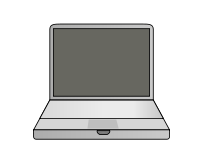
\includegraphics[width=3cm]{images/laptop}};

	\node[mynode, below=2cm of atc] (device2) {Urządzenie 2};
	\node[mynode, left=of device2] (device1) {Urządzenie 1};  	 	 	
	\node[mynode, right=of device2] (device12) {Urządzenie 12};	

	\draw[myline,blue] (laptop.east) -- ++(-1, 0) -- (atc.west);

	\draw[myline] (atc.south) -- (device1.north); 
	\draw[myline] (atc.south) -- (device2.north); 
	\draw[myline] (atc.south) -- (device12.north); 		
	\draw[myline, dotted] (device2.east) -- (device12.west); 	
    
	\draw [fill=blue!5, thick] (-5, -5) rectangle (1, -4);

    \draw [blue, line width=6] (-4.5,-4.5) -- (-4,-4.5); \node at (-3.5,-4.5) {USB};
    \draw [black, line width=6] (-2,-4.5) -- (-1.5,-4.5); \node at (-0.8,-4.5) {RS-485};
\end{tikzpicture} 
\caption{Przykładowa topologia sieci.}
\label{elan:topologia}
\end{figure} % %
\section{Aplikacja ,,GasAnalyzer''}
Oprogramowanie zostało stworzone w całości Javie. Dla ułatwienia kompilacji, zarządzanie zależnościami oraz wersjami zastosowano Apache Maven, które jest narzędziem automatyzującym budowę oprogramowania. Dzięki zastosowanym technologiom projekt można uruchomić na dowolnym komputerze wyposażonym w system operacyjny Windows, Linux lub Mac OXS Cocoa w wersjach 32 i 64 bitowych.

Projekt składa się z dwóch modułów co zostało pokazane na Rysunku~\ref{projectSchema}.Pierwszy z nich ELANNetwork odpowiada za odbieranie danych z sieci, ich weryfikację, przetwarzanie i przekazywanie do warstwy wyższej aplikacji.
Drugi moduł GasAnalyzerGUI jest graficznym interfejsem użytkownika (ang. Graphical User Interface, GUI). Odpowiada za przejrzystą prezentację danych użytkownikowi.

\tikzstyle{abstract}=[rectangle, draw=black, rounded corners, fill=blue!40, drop shadow,
        text centered, anchor=north, text=white, text width=4cm]
\tikzstyle{comment}=[rectangle, draw=black, rounded corners, fill=green, drop shadow,
        text centered, anchor=north, text=white, text width=4cm]
\tikzstyle{myarrow}=[->, >=open triangle 90, thick]
\tikzstyle{line}=[-, thick]

\begin{figure}[!htb] 	
\centering 	
\begin{tikzpicture}[node distance=1.1cm]
    \node (GasAnalyzer) [abstract, rectangle split, rectangle split parts=2]
        {
            \textbf{GasAnalyzer}
            \nodepart{second}wersja 0.1.0
        };
	\node (AuxNode01) [text width=4cm, below=of GasAnalyzer] {};
    \node (ELANNetwork) [abstract, rectangle split, rectangle split parts=2, left=of AuxNode01]
        {
            \textbf{ELANNetwork}
            \nodepart{second}wersja 0.1.0
        };
    \node (GasAnalyzerGUI) [abstract, rectangle split, rectangle split parts=2, right=of AuxNode01]
        {
            \textbf{GasAnalyzerGUI}
            \nodepart{second}wersja 0.1.0
        };    
    \draw[myarrow] (ELANNetwork.north) -- ++(0,0.1) -| (GasAnalyzer.south);
    \draw[line] (ELANNetwork.north) -- ++(0,0.1) -| (GasAnalyzerGUI.north); 
        
\end{tikzpicture}
\caption{Struktura projektu} 
\label{projectSchema}
 \end{figure} %

\subsection{Możliwości}
Aplikacja oferuję mnóstwo przydatnych opcji:
\begin{enumerate}
\item Automatyczne wykrywanie urządzeń podpiętych do sieci,
\item Konfigurowalna precyzja wartości wyświetlanych w GUI i raportach,
\item Bieżący podgląd stanu sieci,
\item Bieżący podgląd stanu każdego urządzenia,
\item Zapis wartości zmierzonych ze wszystkich urządzeń z zadanym interwałem i opcjonalnym komentarzem.
\end{enumerate}

\subsection{Perspektywy}
\begin{enumerate}
\item Implementacja pozostałych możliwości protokołu,
\item Zdalne uruchomienie kalibracji urządzeń,
\item Zdalny odczyt błędów,
\item Rozbudowana detekcja urządzeń (rozpoznanie modelu),
\end{enumerate} %
\section{Bibliografia}
Literatura, która została wykorzystana przez autorów w czasie powstawania projektu, którą opisuje niniejsza dokumentacja.

\begin{thebibliography}{9}
%\begin{enumerate}
%\item 
\bibitem{plc1} 
Jerzy Kasprzyk: 
\emph{"Programowanie sterowników przemysłowych"},
Wydawnictwa Naukowo-Techniczne WNT, 
Warszawa, 
2007      

\bibitem{elan} 
Dokumentacja producenta: 
\emph{„ELAN Interface Description”}, 
sierpień 2006

\bibitem{kurs1} 
Materiały szkoleniowe:
„SIMATIC S7 - Kurs podstawowy”

\end{thebibliography} %

\section{Spis rysunków, tablic i kodów źródłowych}
\subsection{Spis rysunków}
\newlength{\fig}
\settowidth{\fig}{Rysunek\,99:~}
\renewcommand*\numberline[1]{\llap{\makebox[\fig][l]{Rysunek\,#1:~}}}
\makeatletter
\renewcommand*\l@figure[2]{\leftskip\fig\noindent#1\par}
\renewcommand*\l@figure{\@dottedtocline{1}{3cm}{0cm}}
\makeatother
\listoffigures

\subsection{Spis tablic}
%\renewcommand*\numberline[1]{Tablica\,#1: \indent}
\settowidth{\fig}{Tablica\,99:~}
\renewcommand*\numberline[1]{\llap{\makebox[\fig][l]{Tablica\,#1:~}}}
\makeatletter
\renewcommand*\l@table[2]{\leftskip\fig\noindent#1\par}
\renewcommand*\l@table{\@dottedtocline{1}{2.8cm}{0cm}}
\makeatother
\listoftables
\subsection{Spis kodów źródłowych}
\settowidth{\fig}{Kod źródłowy,99:~}
\renewcommand*\numberline[1]{\llap{\makebox[\fig][l]{Kod źródłowy\,#1:~}}}
%\renewcommand*\numberline[1]{Kod źródłowy\,#1:\indent}
\makeatletter
\renewcommand*\l@lstlisting[2]{\leftskip\fig\noindent#1\par}
\renewcommand*\l@lstlisting{\@dottedtocline{1}{4.1cm}{0cm}}
\makeatother
\lstlistoflistings

\end{document}
